\section{System8 Method}
\label{sec:system8}

The System8 method was initialy studied within CMS in~\cite{ref:btag_oldnote}. 
Since then it has been 
improved to include the correlation factors for the Soft Lepton tagger:
 $\delta $ and $\gamma$. In the case of multiple real solutions we have also 
included a criteria to choose the best solution 
when solving the system of equations with an iterative procedure.
 
For the current implementation of the System8 method, 
two data samples are used: the muon-in-jet+away-jet sample, and the 
muon-in-jet+tagged-away-jet sample. The lifetime tag (TrackCounting or 
JetProbability) and the Soft Lepton Tag requiring muon  \ptrel $ > 0.8 $\gevc 
are applied individually or together, and labelled ``tag'', and ``SLT '',
 respectively. The jets are also divided in two categories: 
$b$ jets, and charm+light ($cl$) jets. 

The following system of eight equations is then obtained:

\begin{eqnarray}
n &=& n_b + n_{cl} \nonumber\\
p &=& p_b+ p_{cl} \nonumber\\
n^{\rm{tag}} &=&
\varepsilon_b^{\rm{tag}} n_b + \varepsilon_{cl}^{\rm{tag}} n_{cl} \nonumber\\
p^{\rm{tag}} &=&
\beta \; \varepsilon_b^{\rm{tag}} p_b + \alpha \; \varepsilon_{cl}^{\rm{tag}} p_{cl} \\
n^{SLT} &=&
\varepsilon_b^{SLT} n_b + \varepsilon_{cl}^{SLT} n_{cl} \nonumber \\
p^{SLT} &=& \delta \; \varepsilon_b^{SLT} p_b + \gamma \; \varepsilon_{cl}^{SLT} p_{cl} \nonumber\\
n^{\rm{tag},SLT} &=&
\kappa_b \; \varepsilon_b^{\rm{tag}} \varepsilon_b^{SLT} n_b +
\kappa_{cl} \; \varepsilon_{cl}^{\rm{tag}} \varepsilon_{cl}^{SLT} n_{cl} \nonumber\\
p^{\rm{tag},SLT} &=&
\kappa_b \; \beta \; \delta \; \varepsilon_b^{\rm{tag}} \varepsilon_b^{SLT} p_b +
\kappa_{cl} \; \alpha \; \gamma \; \varepsilon_{cl}^{\rm{tag}} \varepsilon_{cl}^{SLT} p_{cl} \;.\nonumber
\end{eqnarray}

The terms on the left hand side represent the total number of muon-in-jets
in each sample before tagging ($n$, $p$) and after tagging with
a lifetime tagger ($n^{\rm{tag}}, p^{\rm{tag}}$), the soft lepton tagger ($n^{SLT}}, p^{SLT}$), and both ($n^{\rm{tag},SLT},
 p^{\rm{tag},SLT}$). The eight unknowns on the right hand side of the 
equations consist of the number of $b$ and $c+$light jets in the two samples 
($n_b$, $n_{cl}$, $p_b$, $p_{cl}$),  and the tagging efficiencies for
$b$ and $c+$light jets for the lifetime tag and the soft lepton tag
($\varepsilon_b^{\rm{tag}}, \varepsilon_b^{SLT}},
\varepsilon_{cl}^{\rm{tag}}, \varepsilon_{cl}^{SLT}}$).
The method assumes that the efficiency for tagging a jet with both the 
lifetime tag and the  soft lepton tag (muon \ptrel  cut) can be calculated 
as the product of the individual efficiencies.
Six additional parameters are needed to solve the system of equations:
$\kappa_b$, $\kappa_{cl}$, $\alpha$, $\beta$, $\delta$ and $\gamma$. 
The first two parameters represent
the correlation between the lifetime tag and the muon requirement for $b$ jets 
($\kappa_b$) and $c+$light jets ($\kappa_{cl}$), respectively. 
They are defined as
\begin{eqnarray}
\kappa_b = \frac{\varepsilon_b^{\rm{tag},SLT}}
{\varepsilon_b^{\rm{tag}}\varepsilon_b^{SLT}} \;\; {\rm{and}} \;\;
{\kappa_{cl} =
\frac{\varepsilon_{cl}^{\rm{tag},SLT}}{\varepsilon_{cl}^{\rm{tag}}\varepsilon_{cl}^{SLT}}}\,.
\end{eqnarray}

The parameters $\beta$ and $\alpha$ represent the ratio of the lifetime tagging efficiencies
for $b$ and $c+$light jets, respectively, corresponding
to the two data samples used to solve System8.
They are defined as
\begin{eqnarray}
\beta =\frac{ \varepsilon_b^{\mbox{tag}} \mbox{from muon-in-jet+tagged-away-jet sample} } 
{ \varepsilon_b^{\mbox{tag}} \mbox{from muon-in-jet+away-jet sample} }\, ,
\end{eqnarray}
\begin{eqnarray}
\alpha =\frac{ \varepsilon_{cl}^{\mbox{tag}} \mbox{from muon-in-jet+tagged-away-jet sample} } 
{ \varepsilon_{cl}^{\mbox{tag}} \mbox{from muon-in-jet+away-jet sample} }\, .
\end{eqnarray}
And the parameters $\delta$ and $\gamma$ represent the ratio of the soft muon
tagging efficiencies for $b$ and $c+$light jets, respectively, corresponding
to the two data samples used to solve System8.
They are defined as
\begin{eqnarray}
\delta =\frac{ \varepsilon_b^{SLT} \mbox{from muon-in-jet+tagged-away-jet sample} } 
{ \varepsilon_b^{SLT} \mbox{from muon-in-jet+away-jet sample} }\, ,
\end{eqnarray}
\begin{eqnarray}
\gamma =\frac{ \varepsilon_{cl}^{SLT} \mbox{from muon-in-jet+tagged-away-jet sample} } 
{ \varepsilon_{cl}^{SLT} \mbox{from muon-in-jet+away-jet sample} }\, .
\end{eqnarray}

The correlation factors have been measured for three operating points of the 
TrackCounting and the JetProbability tagger and presented in 
Figures~\ref{fig:correlation_TC}-~\ref{fig:correlation_TP}.


\begin{figure}[htbp]
  \begin{center}
    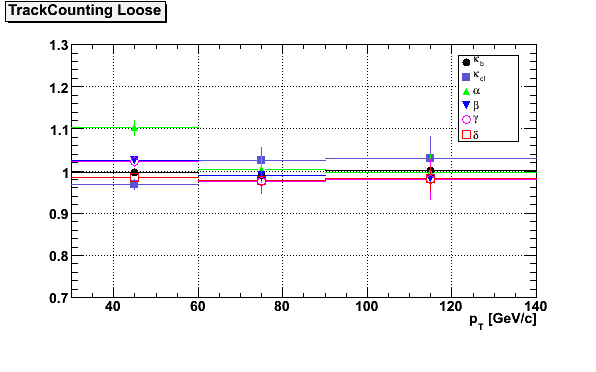
\includegraphics[width=75mm]{Figures/TCL_correlations_ppmux.png}
    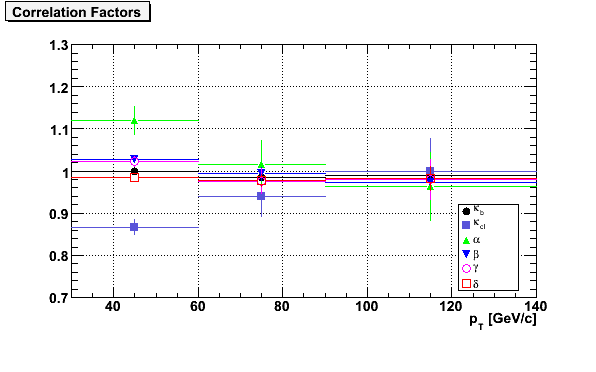
\includegraphics[width=75mm]{Figures/TCM_correlations_ppmux.png}
    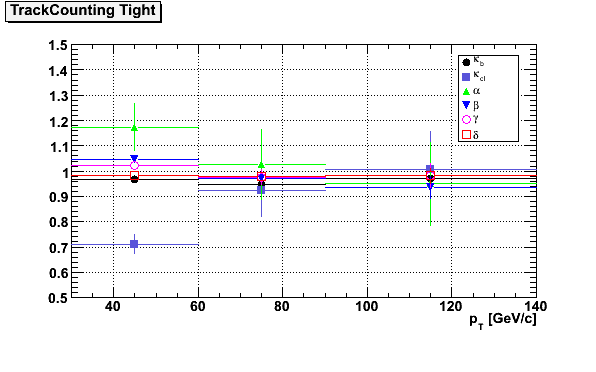
\includegraphics[width=75mm]{Figures/TCT_correlations_ppmux.png}
  \end{center}
  \caption{System8 correlation factors for TrackCounting Tagger as a function
of jet $p_T $ for the loose, medium, and tight operating points for the
$pp\rightarrow $\mu +X$ sample.}
  \label{fig:correlation_TC}
\end{figure}

\begin{figure}[htbp]
  \begin{center}
    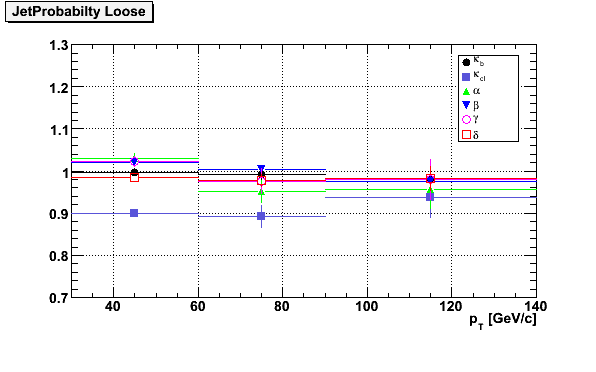
\includegraphics[width=75mm]{Figures/JPL_correlations_ppmux.png}
    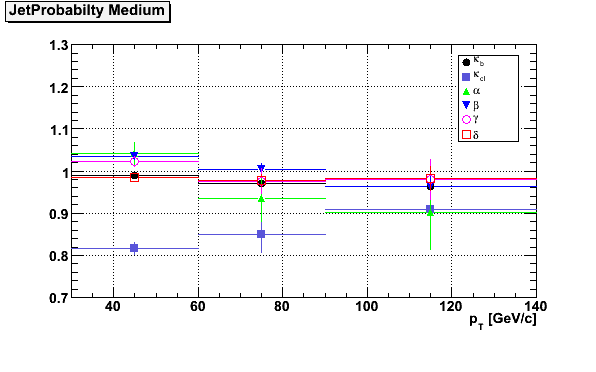
\includegraphics[width=75mm]{Figures/JPM_correlations_ppmux.png}
    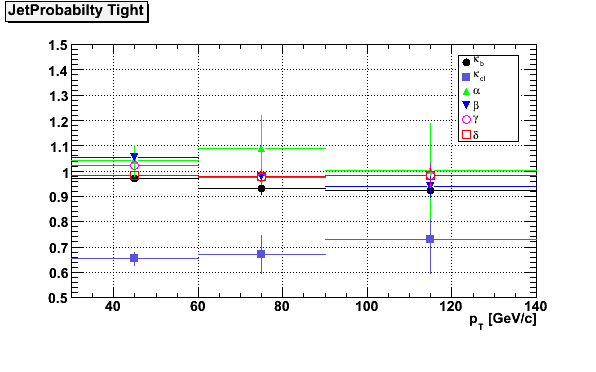
\includegraphics[width=75mm]{Figures/JPT_correlations_ppmux.png}
  \end{center}
  \caption{System8 correlation factors for JetProbability Tagger as a function
of jet $p_T $ for the loose, medium, and tight operating points for the
$pp\rightarrow \mu +X$ sample.}
  \label{fig:correlation_TP}
\end{figure}


